\chapter{系统设计}

\section{框架选型}

\subsection{LeapMotion 与 LeapJS}

LeapMotion \cite{Leap:2016}是一个硬件输入设备和其自身软件的一个总称,
其硬件中内置的两颗深度摄像头和一个红外探测器可以对视野内的手检测,
其软件部分利用内置的骨骼模型对检测的手部进行重新建模,进而完成手行为的高精度
\footnote{ LeapMotion 的官方宣称的识别精度为 0.01mm,
文献\cite{weichert2013analysis, gdu2016} 分析表明 LeapMotion 的实际精度在 0.2 mm 左右。}
识别。

LeapMotion SDK 有两种风格的 API 可以用于获取 LeapMotion 提供的手部数据:
本地接口及 WebSocket 接口,WebSocket 接口便其提供了浏览器环境中的 JavaScipt 接口。
LeapMotion 的 WebSocket 服务遵循 RFC6455
\footnote{\url{http://tools.ietf.org/html/rfc6455}},
运行在连接 LeapMotion 硬件的桌面端的 6437 端口。

而 LeapJS 就是 LeapMotion 控制器的客户端 JavaScript 框架。
使用 LeapJS 可以让 LeapMotion 与网页前端进行通信,此框架可以用来处理接受 LeapMotion JSON 消息。
但随着 NodeJS 的存在,LeapJS 也能够运行在服务端,
因此我们也能够在服务端使用 JavaScript 处理 LeapMotion 消息。

Leap API 以 Frame 为对象,当可被检测的手出现在 LeapMotion 视野内时,
深度摄像头捕捉到的每个 Frame 都能够访问到一个 Hand 对象。
Leap 通过对手部的重新建模,将当前帧的手部信息提供给开发者,
例如当前手的指向、当前手在 LeapMotion 坐标系统下的位置。
借助 LeapMotion 能够省去开发者的手部检测和识别的部分基础工作,更多的关注于手势算法的研究\cite{garber2013gestural,xusuibin2015,panjiajia2015,huhong2015,marin2014hand}。

另外,空间手势已经得到较成熟简单应用,例如文\cite{zaicti2015free}基于 LeapMotion 实现了 TV 上的控制。

\subsection{watchOS 与 WatchConnectivity}

watchOS 是运行在 Apple Watch 上的操作系统。watchOS 刚推出时,
第三方 App 是作为 iOS 的应用扩展存在,手表端只负责对代码的执行结果进行展示,所有的代码都在 iOS 端执行。
随着 watchOS 2 的发布,现在第三方 App 能够通过 WatchConnectivity 框架在 watchOS 和 iOS 之间进行数据通信。

\section{架构设计}
\label{sec:arch-design}

\subsection{通信架构}
\label{sub:im-arch}

watchOS 从 2.0 开始从 iOS App Extension 中剥离开来,将 Watch App 部分全部移至 watchOS 端,
这时这部分代码在手表端具备了可执行的权限,因此将 watchOS 从 1.0 中的单向接收 iOS 端的系统级的通信,
转变为第三方 App 执行管理\cite{WatchGuide:2016},如图 \ref{fig:watch-phone} 所示。
这使其与外界的及时通信成为了可能。

\begin{figure}[H]
    \kaishu
    \centering
    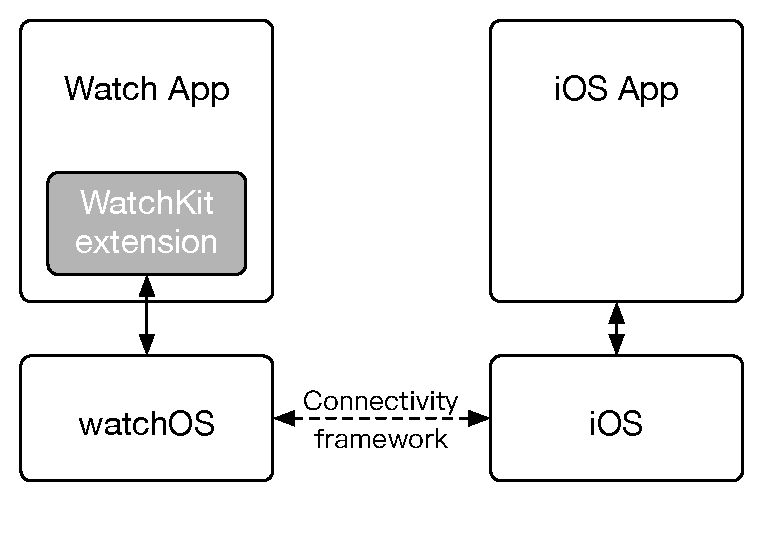
\includegraphics[width=0.4\textwidth]{figures/watch-phone}
    \caption{\kaishu Watch App、WatchKit 扩展和 iOS App 之间的联系}
    \label{fig:watch-phone}
\end{figure}

然而,即便如此在 watchOS 上的网络访问能力依然十分有限,在 watchOS 2 中,
Apple Watch 只能在和与其配对的 iPhone 失去连接,且同时处于已保存的 Wi-Fi 网络覆盖范围内时,
才能独立使用 NSURLSession 访问网络,条件十分苛刻。

鉴于以上考虑,本文对从服务端到客户端的通信架构设计如图 \ref{fig:im-arch} 所示。

\begin{figure}[H]
    \kaishu
    \centering
    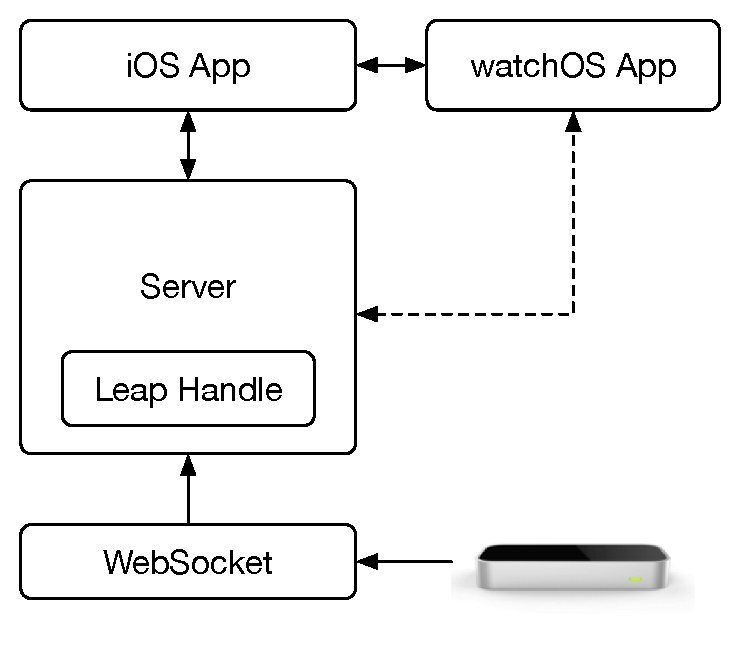
\includegraphics[width=0.4\textwidth]{figures/arch}
    \caption{\kaishu \textbf{通信架构}: watchOS 不直接与服务器进行通信,而是将 iOS 端作为与服务器通信的桥梁}
    \label{fig:im-arch}
\end{figure}

其中,watchOS 将 iOS 端作为与服务器通信的桥梁,处理性能及其有限的 watchOS 端仅负责对通信内容的呈献,
性能稍强的 iOS 端对服务端消息进行筛选与加工,而服务端则对 LeapMotion 原始数据进行分析,
并封装其分析结果后与 iOS 端进行通信。

\subsection{客户端架构}

客户端包含 iOS 端和 watchOS 端两个部分,其架构设计如图 \ref{fig:client-arch} 所示。

\begin{figure}[H]
    \kaishu
    \centering
    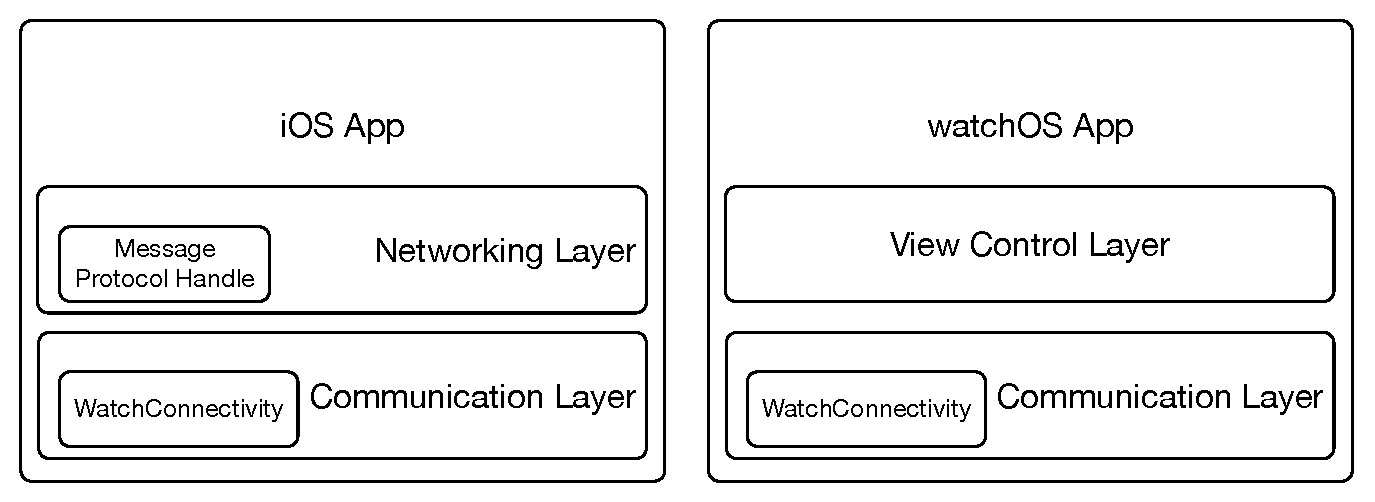
\includegraphics[width=0.6\textwidth]{figures/client-arch}
    \caption{\kaishu \textbf{客户端架构}: iOS 端 App 的网络层对服务器消息进行进一步加工处理,并通过 通信层与 watchOS 进行通信,watchOS 端 App 收到消息后通过视图控制层响应 UI 元素的交互。}
    \label{fig:client-arch}
\end{figure}

\subsection{服务端架构}

服务端的设计如图 \ref{fig:server-arch} 所示,其组件的核心是交互处理层,
该层负责对原始的交互数据进行加工处理为将要实施的交互消息,
然后将加工后的消息按消息协议封装好进而通过请求层分发给相应的请求对象。

\begin{figure}[H]
    \kaishu
    \centering
    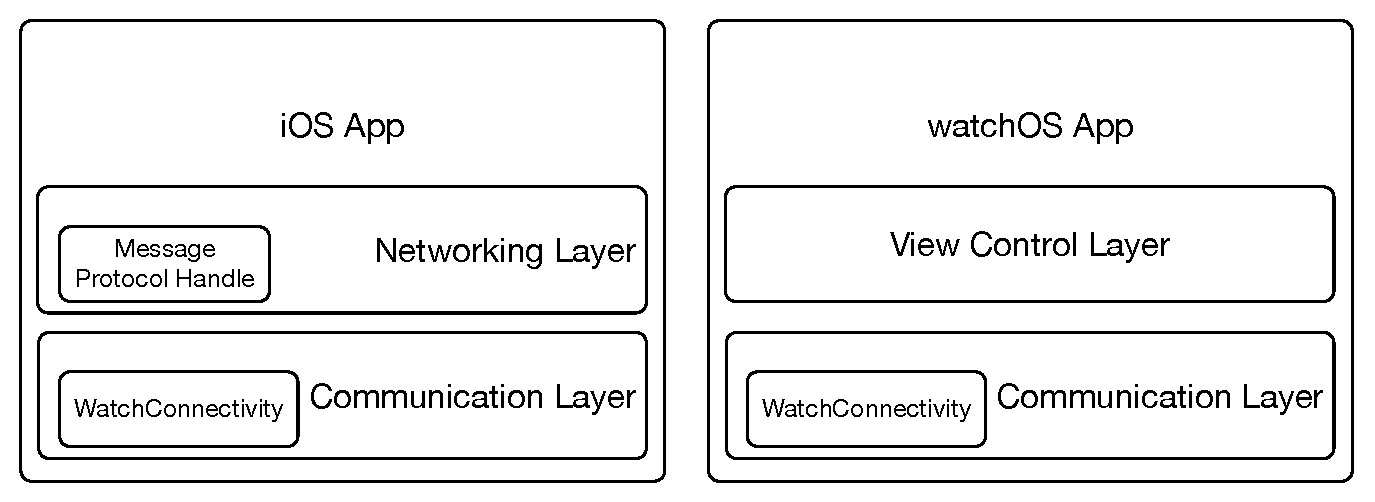
\includegraphics[width=0.6\textwidth]{figures/client-arch}
    \caption{\kaishu \textbf{服务端架构}: 交互处理层对原始数据进行加工处理,完成分析后立即将消息交给请求层并对消息进行分发。}
    \label{fig:server-arch}
\end{figure}

\section{通信协议}

我们需要设计在 watchOS 和 iOS 之间、iOS 与 服务端之间设计相关的交互通信协议。

根据图\ref{fig:interaction}所示,用户与手表端进行交互时共涉及五指合并、双指滑动、手指点击三个基本操作,
其中双指滑动仅指拇指和食指之间的滑动。而对于交互本身的表达,
在图\ref{fig:im-arch}中被设计为由 iOS 端进行表达。
因此,对于服务端与 iOS 端之间的通信数据字段设计如下:

\begin{table}[H]
    %\scriptsize
    \small
    \kaishu
    \centering
    \begin{tabular}{c l l}
        \toprule
        \textbf{返回值字段}        & \textbf{字段类型} & \textbf{字段说明} \\
        \hline
        pinchIndex     & int    & 执行捏合操作的手指,从食指到小指分别为1至4,-1表示当前没有手指进行捏合 \\
        pinchStrength  & double & 拇指与食指捏合的程度,为从0至1连续变化的浮点数 \\
        grabStrength   & double & 五只手指合并的程度,为从0至1连续变化的浮点数 \\
        \bottomrule
    \end{tabular}
    \caption{交互字段说明}
    \label{table:server-feild}
\end{table}

\section{演示程序}

尽管我们对交互方式进行了完备的设计,但由于 Apple Watch 开发上的限制,我们无法对系统级的视图进行操作,因此本文对备择交互一共给出了以下的五个不同效果的演示。

\begin{itemize}
    \kaishu
    \item 第一个演示程序展示了手表点按交互的备择交互设计方案,如图所示;
    \item 第二个演示程序展示了手指在手表屏幕上滑动的备择交互设计方案,如图所示;
    \item 第三个演示程序展示了对 Apple Watch 所特有的 Digital Crown 的备择交互设计,如图所示;
    \item 第四个演示程序展示了对 Apple Watch 所特有的 Force Touch 的备择交互设计方案,如图所示;
    \item 第五个演示程序展示了一个非接触式交互的游戏案例。
\end{itemize}

以上五个演示程序的演示视频可以在 YouTube
\footnote{\url{https://www.youtube.com/playlist?list=PLwUqqMt5en7c2QaQ_DkuvZm9dGTz6RjRM}}
链接中查看,全部相关源代码、环境搭建与演示效果重现的方法可以在 GitHub
\footnote{\url{https://github.com/changkun/BachelorThesis}} 中查看。
